% Original LaTeX code based on Twente Student Conference on IT template

% refers to the cls file being used (ACM standard)
% ACM LaTeX2e Style File V3.2SP
\documentclass{acm_proc_article-sp}

% Allow special chars in sourcecode
\usepackage[utf8]{inputenc}
\usepackage[T1]{fontenc}
\usepackage{lmodern}

\usepackage{xcolor}
\newcommand\todo[1]{\textbf{\textcolor{red}{\uppercase{#1}}}}

\newcommand{\argmin}{\operatornamewithlimits{argmin}}

% Update this if we change the name of the repo
\newcommand\gh{\url{https://github.com/bcleenders/autoTranslate}}

\usepackage{hyperref}

\usepackage{tablefootnote}

% Sample text (test layout)
\usepackage{lipsum}

\begin{document}

\title{Comparing Unsupervised Machine Translation Strategies using Word2Vec}
\subtitle{II2202, Fall 2015}

% Use the \alignauthor commands to handle the names
% and affiliations for an 'aesthetic maximum' of six authors.
% Add names, affiliations, addresses for
% the seventh etc. author(s) as the argument for the
% \additionalauthors command.
% These 'additional authors' will be output/set for you
% without further effort on your part as the last section in
% the body of your article BEFORE References or any Appendices.

\numberofauthors{2} 
\author{
% You can go ahead and credit any number of authors here,
% e.g. one 'row of three' or two rows (consisting of one row of three
% and a second row of one, two or three).
%
% The command \alignauthor (no curly braces needed) should
% precede each author name, affiliation/snail-mail address and
% e-mail address. Additionally, tag each line of
% affiliation/address with \affaddr, and tag the
% e-mail address with \email.
%
% 1st. author
\alignauthor
Bram Leenders\\
       \affaddr{KTH, Royal Institute of Technology}\\
       \affaddr{Brinellvägen 8, 114 28 Stockholm}\\
       \affaddr{Sweden}\\
       \affaddr{\href{mailto:b.c.leenders@gmail.com}{b.c.leenders@gmail.com}}
\alignauthor
Marc Romeyn\\
       \affaddr{KTH, Royal Institute of Technology}\\
       \affaddr{Brinellvägen 8, 114 28 Stockholm}\\
       \affaddr{Sweden}\\
       \affaddr{\href{mailto:marc.romeyn@gmail.com}{marc.romeyn@gmail.com}}
}

\date{\today}

\maketitle
%\begin{abstract}
%Add an abstract or comment this part out
%\end{abstract}

\keywords{Word2Vec, Machine Translation}

\section{Introduction}
\label{sec:introduction}
The Internet offers a vast amount of natural language that can be used in natural language processing, for a very low price. A study by Buck et al.~\cite{buck2014n} estimated that each of the top 10 most frequently used languages on the internet has at least 250 GiB worth of text publically available online. For English (the most frequent), they even found 23 TiB of text.

Such amounts of text have a big potential to be used for the training of language models, but only if building these models can be done in an unsupervised fashion. Manually curating, marking and tagging text is far too much work to be feasible. With unsupervised algorithms, however, the structure in language can be exploited to let computers build language models.

This research will focus on unsupervised training of computer models to translate words. Specifically, we focus on the use of word2vec~\cite{mikolov2013efficient} to provide translations.

\todo{We could expand a bit here, and revisit after writing more of the other parts}

\subsection{Background and Related Work}
\label{sec:prior_work}
Since the introduction of word2vec~\cite{mikolov2013efficient, mikolov2013distributed} in 2013, the algorithm has seen a wide variety of usecases. In the initial paper~\cite{mikolov2013efficient}, Mikolov et. al describe interesting relations between vectors corresponding to words. 
A famous example of how word2vec models relations between words as mathematical equations is $king - man + woman = queen$.
The sematic relationships between man/woman and king/queen are preserved in the transformation of words to vectors, and can be expressed with basic algebra.

Subsequent papers have improved the algorithm both in terms of accuracy (\cite{levy2014linguistic}), performance, parallelization and extended the initial scope of applications. A good example of the latter is a paper by Boycheva~\cite{boycheva2015distributional}, which uses word2vec outside the natural language processing (NLP) domain but to generate playlists. Based on a set of playlists, their word2vec-based algorithm can suggest new playlists with artists that go well together.

One of the applications of word2vec inside the NLP domain, is exploiting similarities in languages for assistance in machine translation~\cite{wolf2014joint}. Mikolov et al.~\cite{mikolov2013exploiting} released a subsequent paper on word2vec, in which they describe similarities between models of different languages. An example they give, is how the usage of the numbers one to five in English is very similar to the usage in Spanish, and likewise for the names of animals. Figure~\ref{fig:english_spanish} shows a graphical representation of word vectors in English and Spanish.

\begin{figure}[ht!]
  \centering 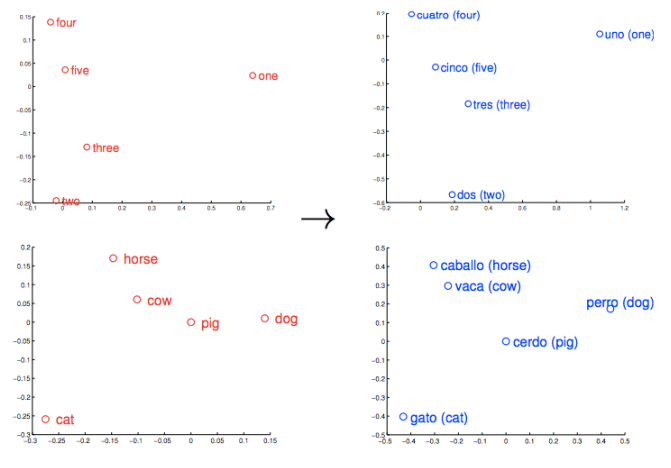
\includegraphics[width=\linewidth]{images/english_spanish}
  \caption{Vector representations of English and Spanish words, after dimensionality reduction and rotation. Notice the high level of similarity between both languages. Reprinted from Mikolov et al.~\cite{mikolov2013exploiting}}
  \label{fig:english_spanish}
\end{figure}

The similarities between languages can be used to predict translations for words without any human interaction or labeled input data. Using only unsupervised machine learning techniques, a computer could learn how to translate English to for instance Spanish and vice versa. The only requirement is a large amount of text in both languages to train the word2vec models on.

In this research, we will focus on this specific application of word2vec: using similarities in languages to provide translations of words.

It is important to note that word2vec only uses information of co-occurrences to model words. It does not learn grammatical concepts other than by statistical analysis. This limits our translation to single words; although the translator might be able to translate each word individually, it cannot learn that each finite verb must has a subject, that "we" is plural, etc. It will learn that "swim" is to "swimming" as "walk" is to "walking", but will not know that "swimming" is a gerund. Note that word2vec can be extended to sentences or whole documents as proposed by Le et al.~\cite{le2014distributed} but this will be out of scope for our research.

\subsection{Our Contribution}
This research aims to improve the capabilities of machines to learn translations with minimal human intervention. Previous research~\cite{mikolov2013exploiting, wolf2014joint} has already shown potential for word2vec in the context of automatic translation, as discussed in section~\ref{sec:prior_work}.

However, we found no practical implementations using Word2Vec and no further research on different setups for word2vec based machine translation.

\subsection{Outline}
\todo{Briefly explain structure of paper}

\subsection{Word2Vec}
Word2Vec is an algorithm that computes vector representations of words based on co-occurrences. The spatial distance between two word-vectors corresponds to word similarity. In order to achieve this there two different algorithms: skip-gram and continuous bag of words (CBOW). Skip-gram is the most popular choice because it scales better to bigger datasets and therefore also chosen for our research. 

Skip-gram model is an method for learning distributed vector representations that capture a large number of syntactic and semantic word relationships \cite{mikolov2013distributed}. Given a a word $w$, the skip-gram model predicts the $n$ neighboring words.

Word2Vec is an example of ''shallow" learning and can be trained as a simple neural network. This neural network has a single hidden layer with no non-linearities and no unsupervised pre-training of layers is needed \cite{wang2014introduction}. 
\section{Relations Between Languages}
\label{sec:relations}
\todo{Explain how king is to koning as queen is to koningin}

:) is to :( as happy is to sad

... etc.
\section{Multi-model Translations}
\label{sec:multi-model-translations}
In this section, we explain a technique for translating words using seperate models for the input and output language. The techniques described here are originally published by Mikolov et al.~\cite{mikolov2013exploiting}.

\subsection{Translation}
Given a word in language A that we want to translate to language B, the first step is to find the vector representation of the word. We do this by looking up the word in a word2vec model trained on language A.

Translating is now a matter of mapping vector representations from model A to corresponding vectors in model B. We do this by multiplying the vector with a translation matrix, which gives an expected vector in model B.

The last step is to convert the "translated" vector representation back to a word. We do this by looking up which word in language B which has the vector representation closest to the translated vector. The criterium used for this is simply nearest neighbour with a Euclidean distance.

\subsection{Training the Models}
This way of translation requires three models: word2vec models for both language A and B and a translation matrix from A to B.

The two language models are trained using the default word2vec algorithm. We refer to previous papers for the specifics on this \cite{mikolov2013efficient, mikolov2013distributed}.

The translation matrix is trained by solving the following expression:
$$ \argmin_{T} \Sigma_{i=1}^{n} || T \cdot a_i - b_i || ^{2}$$
where $T$ is an $n$ by $n$ matrix, $a_i$ and $b_i$ are $n$ dimensional vector representations of words in languages A and B, such that $b_i$ is the translation of $a_i$.

The quality of the translation largely depends on the accuracy of the mapping from vectors in model A to model B. Training language models using word2vec is unsupervised, and can therefore use hundreds of gigabytes or even terabytes of training data. Training the translation matrix is a supervised process (you have to provide correct translations), which makes it impractical to provide more than a few thousand words.

An advantage of using this method, is that it not only provides a word translation but also gives a distance between the translated vector and its nearest neighbour. If this distance is large, it indicates a higher level of uncertainty in the matrix. As such, one can search for potential bad translations and provide targeted training data to improve a next iteration of the model.

\subsection{Training models of different sizes}
One of the parameters when training word2vec models is the number of dimensions to train on. Typically, the number of dimensions is between 100 and 400\cite{mikolov2013efficient}.

Large datasets contain many relations, and can be trained on high dimensions (400 or more), but small datasets (i.e. under 50 million words) tend to be trained with lower dimensionality. However, these numbers are not set in stone: a study by Pennington et al.~\cite{jeffreypennington2014glove} indicates that 300 dimensions sufficiently capture relations -for their dataset. Since training complexity scales linearly with the number of dimensions, for very large datasets a high dimensionality might even simply be too costly.

Having discussed the cost/benefit of higher dimensions, we remark that translations with multiple models also allows for models trained with a different number of dimensions. If both models have the same dimensions, the translation matrix will be square. If the dimensions are different, one can either use dimensionality reduction on the larger matrix, or use a non-square translation matrix to scale down the dimensionality.
\section{Single-model Translations}
\label{sec:single-model-translations}

\subsection{Translation using Relations}
\label{sec:single-model-no-matrix}
As a simplest form of translation, one could say that "king" is to "koning" (the Dutch word for king) as "queen" is to "koninging" (Dutch for queen). Intuitively, this means we consider relations between two languages, instead of relations within a single language.

Thus, if we train a single model with two languages in it, one could expect to find these relations and use them to translate Dutch to English and vice versa.

This method is so simplistic, we do not expect it to give good translations. There is no guarantee the trained model models the Dutch-English relation in a consistent manner. A proper English sentence will not contain the word "koning", since it is not an English word. As such, it will be difficult (if not impossible) for word2vec to learn that "koning" and "king" are related.

Despite our doubts about its effectiveness, we choose to include this method as a baseline for performance and simplicity. Any more complex method performing not at least as good as this is not worth the additional complexity.

\subsection{Translation matrix in single space}
\label{sec:single-model-with-matrix}
A mix between the two methods described above is using a single model trained on multiple languages (as in the previous section), but using a translation matrix (as in section~\ref{sec:multi-model-translations}).

This method would allow the language model to be trained without having to take into account the languages it is being trained on. As such, one could feed it text without determining the language that text is written in. This is a significant advantage for applications where the input is unlabelled.

\section{Experiments}
\label{sec:experiments}

\subsection{Datasets}
The datasets used to train the word2vec models are freely available online. We used the wikipedia datasets containing a snapshot of all articles on the English and Dutch Wikipedia and a copy of all Reddit comments.

The Go program used for cleaning the Reddit data is published on GitHub\footnote{\gh}. The wikipedia data was parsed with a slightly modified version of Wikipedia Extractor\footnote{\url{https://github.com/bwbaugh/wikipedia-extractor}}, which is also available on our GitHub page.

The characteristics of the cleaned datasets can be seen in table~\ref{table:datasets}.

%
% Get these statistics with:
% wc -w <files>		for the wordcount. Do it on the extracted, processed text (i.e. the input for word2vec)
% Number of items: see end of running wikiextractor.py
% e.g. INFO: Finished 31-process extraction of 1831031 articles in 11250.7s (162.7 art/s)
%
\begin{table}[ht!]
	\centering
	\label{table:datasets}
	\begin{tabular}{|l|c|r|r|}
	\hline
	Name																												& Items			& Words			\\
	\hline
	Reddit comments \tablefootnote{\url{http://academictorrents.com/details/7690f71ea949b868080401c749e878f98de34d3d}} 	& 1,325,482,268 & 38,177,224,313\\
	English Wikipedia \tablefootnote{\url{https://dumps.wikimedia.org/enwiki/20150901/}}								& 4,929,936		& 1,707,791,444	\\
	Dutch Wikipedia \tablefootnote{\url{https://dumps.wikimedia.org/nlwiki/20150901/}}									& 1,831,031		& 209,095,532	\\
	\hline
	\end{tabular}
	\caption{Dataset statistics. For Wikipedia, "Items" refers to the number of articles. For Reddit, it refers to the number of comments.}
\end{table}

\subsection{Tests}
We tested each translation method in multiple configurations, most notably with different dimensions for the language models.

The accuracy of the translation is measured in percentages how often the algorithm gave the expected answer. To account for answers that are almost correct, we keep the following statistics:
\begin{itemize}
	\item \textbf{Accuracy @1}: the algorithm gave the correct answer.
	\item \textbf{Accuracy @5}: the correct answer was in the top 5.
	\item \textbf{Accuracy @10}: the correct answer was in the top 10.
\end{itemize}

If the answer is in the top 5 it is likely to be a synonym or very related word, since word2vec tends to group words by meaning. For example, the translation may be "buy" or "acquire" where the correct translation is "purchase".

Each test is repeated 10 times with a randomly chosen training and test dataset to provide cross-validation. The results given in the next section are the averages of the tests.
\section{Results}
\label{sec:results}

\todo{Add more results (matter of running more experiments, mostly)}

\subsection{Multi-model Translations}
Figure~\ref{fig:accuracy_multi_model_wikis} shows the accuracy of the multi-model translations, both for models trained on 100 and 400 dimensions. We used the same training set of translations to train the matrix on, and both language models are trained on respectively the Dutch and English Wikipedia.

An interesting observation is that the accuracy at all levels (top 1, top 5 and top 10) starts off lower for models trained at 400 dimensions. However, at the biggest training set, each level is better than the corresponding level at 100 dimensions. This suggests a form of overfitting; the translation matrix might be overfitted on the translation samples.

\todo{There's also a dip towards the end. Check if that's still there if we run it with differently split test/training data sets.}

\begin{figure}[ht!]
  \centering 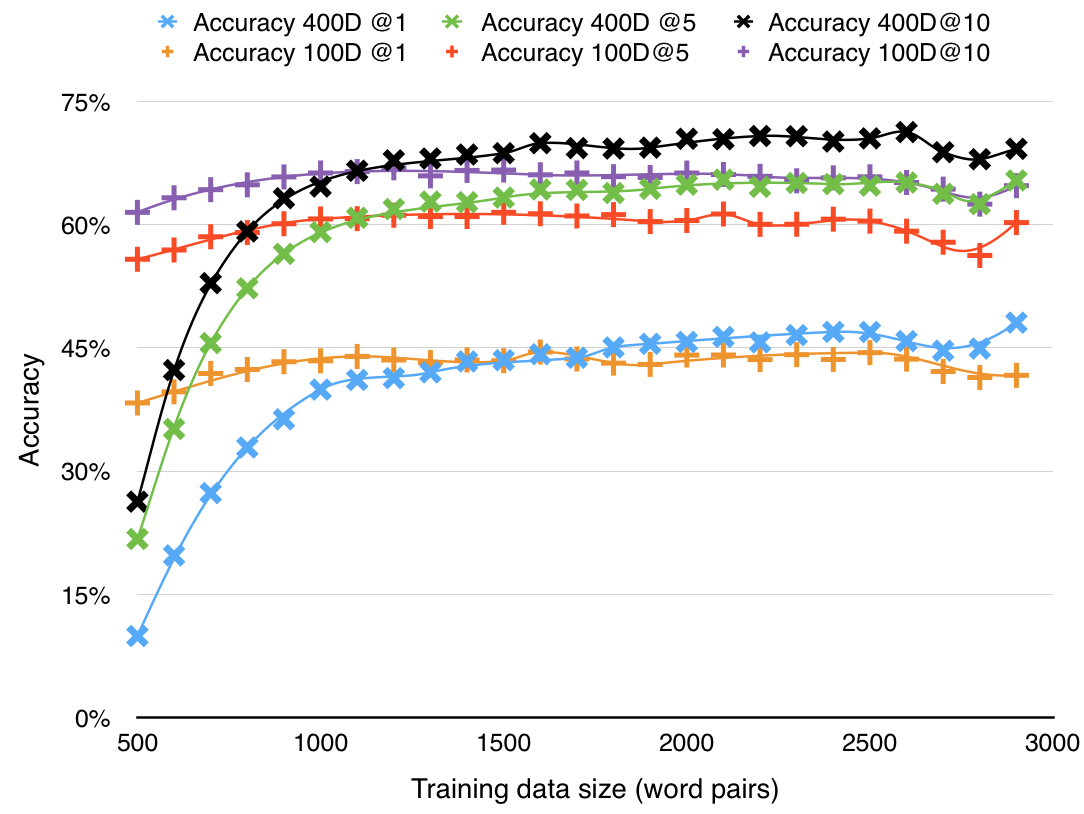
\includegraphics[width=\linewidth]{images/accuracy_multi_model_wikis}
  \caption{Accuracy for multi-model translations, trained on Dutch and English wiki. 'x' marks denote dimensionality 400, '+' marks dimensionalty 100.}
  \label{fig:accuracy_multi_model_wikis}
\end{figure}

\subsection{Single-model Translations}
In this section, we use two models: both are trained on the text of the English Wikipedia and the Dutch Wikipedia combined. Since the Dutch Wikipedia is much smaller than its English counterpart (by a factor of 8, see table~\ref{table:datasets}), we ran it eight times over the Dutch text. This artificially increases the weight given to Dutch text, so both are equally well represented.

The only difference between the two models is the number of dimensions: one is trained at 100, and the other at 400 dimensions.

\subsubsection{Using Relations}
The method described in section~\ref{sec:single-model-no-matrix} is tested by randomly selecting 100 translations from our testset of correct translations. These are used as a known translation, to derive other translations from. For each of these translations, we then select 500 different translations to test against. This process is done both for a model trained at 100 dimensions, and one trained at 400 dimensions, and both for Dutch to English and vice versa.

For example, given "koning $\to$ king" as base pair, we then test whether the algorithm can translate "koningin" to "queen", "kopen" to "buy", et cetera.

Table~\ref{table:results_single_model_no_matrix} shows the results of these experiments.

\begin{table}[ht!]
  \centering
  \label{table:results_single_model_no_matrix}
  \begin{tabular}{ll|r|r|r|r|}
  \cline{3-6}                                       &     & \multicolumn{2}{|c|}{100 dim} & \multicolumn{2}{c|}{400 dim} \\ \cline{3-6} 
                                                    &     & NL$\to$EN   & EN$\to$NL       & NL$\to$EN   & EN$\to$NL      \\ \hline
    \multicolumn{1}{|l|}{\multirow{3}{*}{Avg.}}     & @1  & 4.29\%      & 3.92\%          & 1.91\%      & 2.02\%         \\ \cline{2-6} 
    \multicolumn{1}{|l|}{}                          & @5  & 8.71\%      & 8.28\%          & 4.89\%      & 4.97\%         \\ \cline{2-6} 
    \multicolumn{1}{|l|}{}                          & @10 & 11.4\%      & 10.9\%          & 6.96\%      & 7.00\%         \\ \hline 
    \multicolumn{1}{|l|}{\multirow{3}{*}{Max.}}     & @1  & 14.6\%      & 12.4\%          & 8.60\%      & 8.60\%         \\ \cline{2-6} 
    \multicolumn{1}{|l|}{}                          & @5  & 23.4\%      & 23.8\%          & 15.8\%      & 16.4\%         \\ \cline{2-6} 
    \multicolumn{1}{|l|}{}                          & @10 & 28.4\%      & 28.6\%          & 21.2\%      & 22.0\%         \\ \hline
    \multicolumn{1}{|l|}{\multirow{3}{*}{Stdev.}}   & @1  & 3.50\%      & 3.24\%          & 1.97\%      & 2.19\%         \\ \cline{2-6} 
    \multicolumn{1}{|l|}{}                          & @5  & 6.10\%      & 6.15\%          & 4.11\%      & 4.55\%         \\ \cline{2-6} 
    \multicolumn{1}{|l|}{}                          & @10 & 7.51\%      & 7.60\%          & 5.42\%      & 5.85\%         \\ \hline
  \end{tabular}
  \caption{Translation accuracy, using a single model without translation matrix and 400 dimensions. The minimum is left out, because it is 0.00\% for all scenarios.}
\end{table}

An interesting note (which is not shown in the table), is that for every scenario, the lowest percentage of correct translations is 0.00\%. This means that there are some very bad base translations. In the next section, we will give some reasons what may cause this.

\subsubsection{Using Translation Matrix}
Check figure \ref{fig:accuracy_single_model_wikis} for the results.

Again: weird dip towards the end. \todo{Marc, do you know why? Just bad luck choosing test samples?}

\begin{figure}[ht!]
  \centering 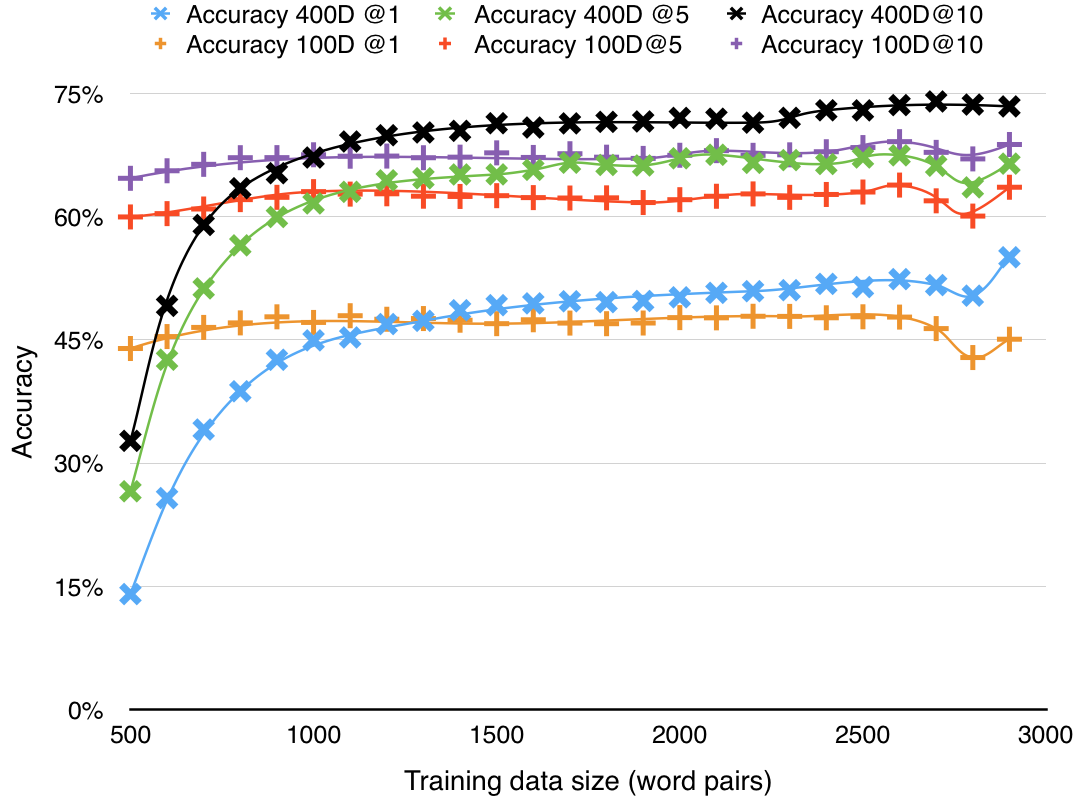
\includegraphics[width=\linewidth]{images/accuracy_single_model_wikis}
  \caption{Accuracy for multi-model translations, trained on Dutch and English wiki. 'x' marks denote dimensionality 400, '+' marks dimensionalty 100.}
  \label{fig:accuracy_single_model_wikis}
\end{figure}

\section*{Acknowledgements}
The authors thank SICS Swedish ICT for the resources they provided.

%References
\bibliographystyle{abbrv}
\bibliography{references}

\balancecolumns
\end{document}